\documentclass[11pt,a4paper]{article}
\usepackage[document]{ragged2e}
\usepackage{polski}
%\usepackage[cp1250]{inputenc}
\usepackage{titlesec}
\titlelabel{\thetitle.\quad}
\usepackage{amsmath}
\usepackage{graphicx}
\usepackage{float}
\usepackage[T1]{fontenc}
\usepackage{longtable}
\usepackage[nottoc, notlof, notlot]{tocbibind} 
%\usepackage[nottoc, nobib]{natbib}
\usepackage[colorinlistoftodos]{todonotes}
\usepackage{lineno}
\usepackage{listings}
\usepackage{xcolor} % Do kolorów
\usepackage[hidelinks]{hyperref} % ukrycie kolorowych prostokatow otaczajacych linki
\setlength {\marginparwidth }{2cm}
\newcommand{\dd}[1]{\mathrm{d}#1}
\renewcommand{\figurename}{Rys.}
\renewcommand{\tablename}{Tab.}
\renewcommand{\listfigurename}{}
\renewcommand{\listtablename}{}
\renewcommand{\lstlistlistingname}{}
%\renewcommand{\bibname}{}
%\usepackage[notocbib]{apacite}
\usepackage{geometry}

\geometry{
	a4paper,
	total={170mm,257mm},
	left=25mm,
	top=20mm,
}
\usepackage[
open,
openlevel=2,
atend,
numbered, 
]{bookmark}

\graphicspath{{./graphic}}

\usepackage{color}
\definecolor{mygreen}{rgb}{0,0.6,0}
\definecolor{mygray}{rgb}{0.5,0.5,0.5}
\definecolor{mymauve}{rgb}{0.58,0,0.82}

\lstset{ 
	backgroundcolor=\color{white},   % choose the background color; you must add \usepackage{color} or \usepackage{xcolor}; should come as last argument
	basicstyle=\footnotesize,        % the size of the fonts that are used for the code
	breakatwhitespace=false,         % sets if automatic breaks should only happen at whitespace
	breaklines=true,                 % sets automatic line breaking
	captionpos=t,                    % sets the caption-position to bottom
	commentstyle=\color{mygreen},    % comment style
	deletekeywords={...},            % if you want to delete keywords from the given language
	escapeinside={\%*}{*)},          % if you want to add LaTeX within your code
	extendedchars=true,              % lets you use non-ASCII characters; for 8-bits encodings only, does not work with UTF-8
	firstnumber=1,                % start line enumeration with line 1000
	frame=single,	                   % adds a frame around the code
	keepspaces=true,                 % keeps spaces in text, useful for keeping indentation of code (possibly needs columns=flexible)
	keywordstyle=\color{blue},       % keyword style
	language=Octave,                 % the language of the code
	morekeywords={*,...},            % if you want to add more keywords to the set
	numbers=left,                    % where to put the line-numbers; possible values are (none, left, right)
	numbersep=5pt,                   % how far the line-numbers are from the code
	numberstyle=\tiny\color{mygray}, % the style that is used for the line-numbers
	rulecolor=\color{black},         % if not set, the frame-color may be changed on line-breaks within not-black text (e.g. comments (green here))
	showspaces=false,                % show spaces everywhere adding particular underscores; it overrides 'showstringspaces'
	showstringspaces=false,          % underline spaces within strings only
	showtabs=false,                  % show tabs within strings adding particular underscores
	stepnumber=2,                    % the step between two line-numbers. If it's 1, each line will be numbered
	stringstyle=\color{mymauve},     % string literal style
	tabsize=2,	                   % sets default tabsize to 2 spaces
	title=\lstname                   % show the filename of files included with \lstinputlisting; also try caption instead of title
}

\usepackage{hyperref} % Pakiet do ustawiania metadanych PDF


\title{
	{\Huge Politechnika Warszawska  \\[1\baselineskip]} 
	{\huge Wydział Elektryczny \\[1\baselineskip]
		Instytut Sterowania i Elektroniki Przemysłowej 	\\[2\baselineskip]}	
	Sprawozdanie z projektu „Wielowątkowość wysokopoziomowa" \\[2\baselineskip]
	
	\begin{figure}[!htb]
		\centering
		
\includegraphics[width=0.3\textwidth]{logopw.png}
	\end{figure}
	
	\begin{center}
    \vspace*{\fill}
    \Large
    \begin{tabular}{lr}
        Michał Bobrycki & 331 766 \\
        Karol Cegliński & 331 773 \\
        Przemysław Cichoń & 331 775 \\
        Tomasz Rachwał & 331 796 \\
        Kacper Zawadka & 331 813
    \end{tabular}
    \vspace*{\fill}	
\end{center}
	
}

\begin{document}
	\justifying
	\maketitle
	
	\vspace*{\fill}	
	\begin{flushright}
		Prowadzący: dr hab. inż. Dominik Olszewski 
	\end{flushright}
    \newpage
	\tableofcontents % spis tresci
    \newpage
    %=================================================
    %=================================================
    \newpage\section{Cel projektu}
Głównym celem projektu było zapoznanie się z podejściem wysokopoziomowym do tworzenia wątków i zarządzania nimi w języku Java. Projekt wymagał zaimplementowania aplikacji graficznej (animacji), w której wiele elementów porusza się równocześnie, oraz przeprowadzenia analizy porównawczej między klasyczną techniką wykorzystującą interfejs \texttt{Runnable} i klasę \texttt{Thread}, a metodami z pakietu \texttt{java.util.concurrent} (\texttt{Executor}, \texttt{ExecutorService}, \texttt{ScheduledExecutorService}).

\newpage\section{Opis struktury kodu i implementacji}
Aplikacja została napisana z wykorzystaniem biblioteki Swing i składa się z kilku kluczowych klas i segmentów:

\begin{itemize}
    \item \textbf{\texttt{ThreadingProject\_P1}}: Klasa główna, definiująca parametry brzegowe, takie jak liczba elementów (100) oraz rozmiar puli wątków (4). Uruchamia ona GUI w bezpiecznym wątku \texttt{Event Dispatch Thread} za pomocą \texttt{SwingUtilities.invokeLater}.
    \item \textbf{\texttt{Animacja}}: Główna klasa zarządzająca oknem (dziedzicząca po \texttt{JFrame}). Zawiera metody podpięte pod przyciski interfejsu, z których każda inicjuje ruch obiektów za pomocą innej techniki wielowątkowej. Klasa ta zawiera również metodę \texttt{heavyCalculations()}, która za pomocą operacji trygonometrycznych sztucznie obciąża procesor, symulując złożone obliczeniowo zadanie.
    \item \textbf{\texttt{KrokAnimacji}}: Implementacja interfejsu \texttt{Runnable}. W metodzie \texttt{run()} zaimplementowano pętlę \texttt{while}, która wykonuje ciężkie obliczenia, przesuwa klocek w prawo i odświeża interfejs tak długo, aż klocek dotrze do prawej krawędzi okna.
    \item \textbf{\texttt{PanelAnimacji} i \texttt{RuchomyElement}}: Klasy odpowiedzialne za warstwę wizualną. \texttt{PanelAnimacji} przechowuje listę klocków (\texttt{CopyOnWriteArrayList} dla bezpieczeństwa wątkowego) i odpowiada za ich rysowanie, natomiast \texttt{RuchomyElement} to prosta struktura przechowująca współrzędne X i Y.
\end{itemize}

\newpage\section{Porównanie wykorzystanych metod wielowątkowości}

W projekcie wykorzystano cztery podejścia do uruchamiania zadań. Na podstawie analizy teoretycznej oraz budowy poszczególnych interfejsów, można je scharakteryzować następująco:

\begin{description}
    \item[Runnable + Thread ] \hfill \\
    Opiera się na ręcznym tworzeniu i uruchamianiu każdego wątku z osobna (\texttt{new Thread(...).start()}). System operacyjny musi powołać nowy, fizyczny wątek dla każdego zadania, co przy dużej ich liczbie (w tym przypadku 100) drastycznie obciąża procesor i pamięć ze względu na koszt tzw. przełączania kontekstu. Brakuje tu mechanizmów zarządzania pulą i reużywalności zasobów.
    
    \item[Executor] \hfill \\
    Najprostszy interfejs z pakietu \texttt{java.util.concurrent}. Oddziela definicję zadania od mechanizmu jego uruchomienia, udostępniając jedynie metodę \texttt{execute()}. W implementacji projektu użyto krótkiego zapisu, który w tle inicjuje i uruchamia klasyczny wątek. Jest to interfejs nie dający kontroli nad cyklem życia wątków ani nie pozwalający wprost sprawdzić statusu zakończenia zadania.
    
    \item[ExecutorService] \hfill \\
    Rozbudowana wersja interfejsu \texttt{Executor}, w projekcie zaimplementowana jako stała pula wątków (\texttt{Executors.newFixedThreadPool(4)}). Pula składa się ze stałej grupy przypisanych wątków, które wielokrotnie pobierają kolejne zadania z kolejki. Zapewnia to pełną kontrolę nad cyklem życia (np. ułatwione zatrzymywanie przez \texttt{shutdownNow()}). Mechanizm ten w dużym stopniu oszczędza zasoby komputera, ponieważ unika ciągłego tworzenia i niszczenia obiektów \texttt{Thread}.
    
    \item[ScheduledExecutorService] \hfill \\
    Rozszerza możliwości \texttt{ExecutorService} o wbudowany harmonogram. Zamiast wykonywać zadania od razu i w ciągłej pętli, pozwala na ich opóźnienie lub precyzyjne, cykliczne powtarzanie (\texttt{scheduleAtFixedRate}). W projekcie zastępuje to ręczne usypianie wątków (\texttt{Thread.sleep()}) oraz usuwa potrzebę stosowania pętli \texttt{while} w samym zadaniu, przenosząc logikę powtarzania na poziom zarządcy (frameworku).
\end{description}

\newpage\section{Analiza wyników i zachowania animacji}

Obserwacja zachowania wizualnego klocków (reprezentujących wątki) w interfejsie graficznym doskonale odzwierciedla mechanikę działania poszczególnych podejść do wielowątkowości:

\begin{itemize}
    \item \textbf{Thread + Runnable:} Wszystkie 100 klocków rusza jednocześnie, jednak ich ruch jest bardzo nieregularny, a wręcz losowy. Nie idą w partiach, ulegają rozproszeniu i stale przesuwają się względem siebie. Wynika to z faktu, że planista systemu operacyjnego (OS scheduler) musi sprawiedliwie rozdzielić czas procesora między 100 aktywnych, ciężkich fizycznych wątków, co prowadzi do nierównomiernego dostępu do CPU.
    
    \item \textbf{Executor:} Przebieg animacji wygląda niemal identycznie jak w podejściu klasycznym. Wynika to z użytej implementacji interfejsu \texttt{Executor} (\texttt{command -> new Thread(command).start()}), która de facto zachowuje się pod spodem tak samo jak bezpośrednie użycie \texttt{Thread}.
    
    \item \textbf{ExecutorService (pula 4 wątków):} Klocki poruszają się wyraźnymi partiami (po 4 sztuki naraz). Wynika to z faktu, że pętla \texttt{while} w obiekcie \texttt{KrokAnimacji} „blokuje” wątek z puli aż do momentu, gdy klocek dotrze do mety. Dopiero po zakończeniu całego biegu klocka, wątek z puli jest zwalniany i pobiera z kolejki kolejne zadanie (kolejny klocek). Niewielkie przesunięcia wewnątrz poruszających się klocków wynikają z faktu, że wątki nadal muszą konkurować o zasoby systemowe.
    
    \item \textbf{ScheduledExecutorService:} Wszystkie klocki przemieszczają się niemal w jednej pionowej linii w sposób równomierny i falowy. To diametralnie inne zachowanie wynika ze zmiany struktury wywołania. Zamiast ciągłej pętli \texttt{while} dla każdego klocka, do planisty wrzucono 100 krótkich zadań (jeden skok o 2 piksele), które wykonują się co 10 milisekund z wykorzystaniem puli 4 wątków. Pula 4 wątków jest w stanie błyskawicznie obsłużyć 100 mikrozadań w ramach pojedynczego cyklu co 10ms, dzięki czemu klocki przesuwają się synchronicznie.
\end{itemize}

\newpage\section{Analiza z wykorzystaniem profilera}

Na poniższym zrzucie ekranu zaprezentowano przebiegi analizujące wpływ działającego programu na zachowanie CPU oraz wątków.
\begin{figure}[H]
    \centering
    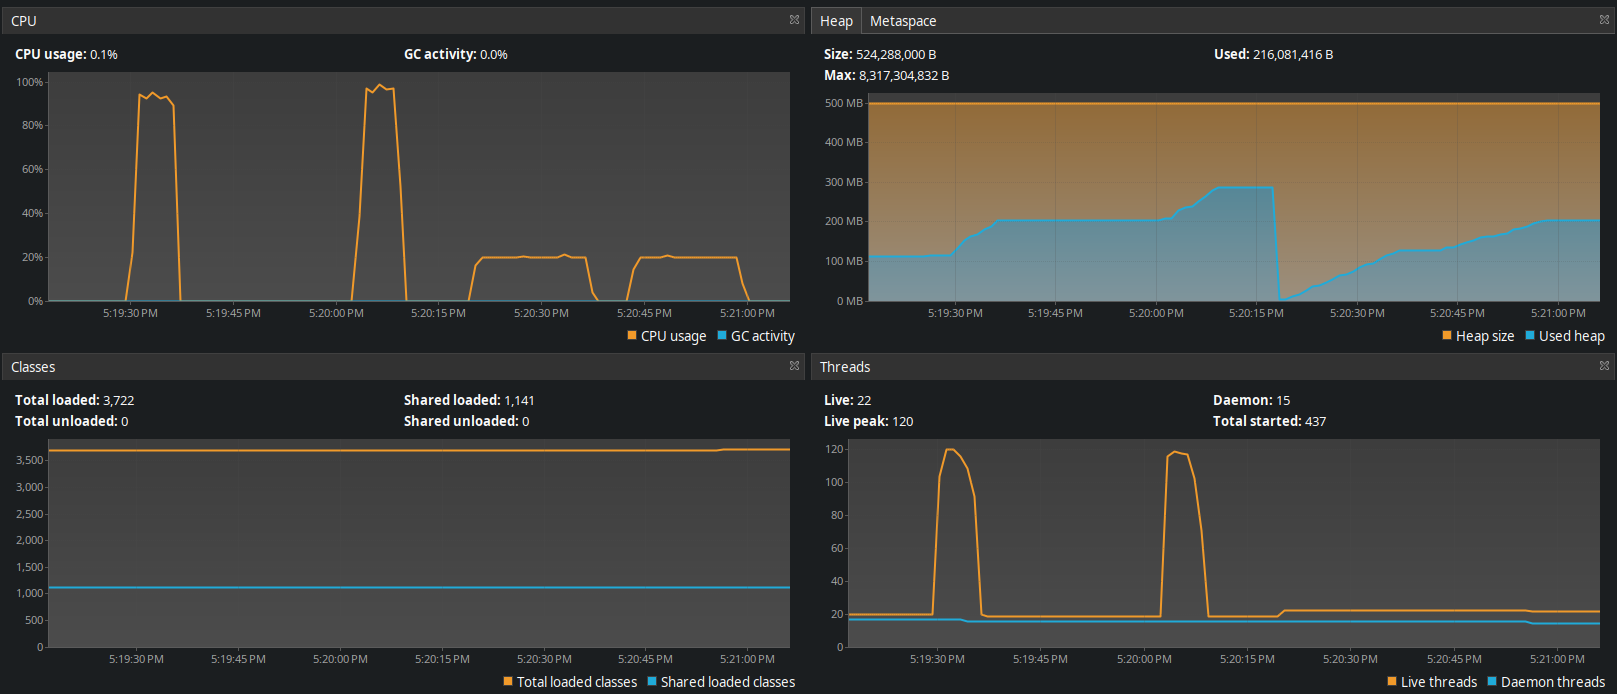
\includegraphics[width=1\linewidth]{image3143.png}
    \caption{Analiza działania aplikacji z wykorzystaniem profilera}
\end{figure}


\begin{itemize}
    \item \textbf{Technika klasyczna (Thread + Runnable):} 
    Pierwszy skrajnie wysoki pik po lewej. Charakteryzuje się bardzo krótkim czasem wykonania (wąski słupek), ale ogromnym kosztem zasobów -- zużycie CPU sięga blisko 100\%, a liczba aktywnych wątków skacze do około 120 (tworzony jest nowy fizyczny wątek dla każdego klocka). Takie działąnie powoduje, że klocki na ekranie przesuwają się nieregularnie i chaotycznie.

    \item \textbf{Podstawowy Executor:} 
    Drugi wysoki pik na wykresie. Wykazuje parametry zużycia zasobów (CPU i skok liczby wątków) i czas wykonania w zasadzie identyczne jak podejście pierwsze. Każdorazowo tworzony jest nowy wątek. Odzwierciedla to animacja, która wizualnie zachowuje się tak samo niestabilnie jak przy metodzie klasycznej.

    \item \textbf{Podejście wysokopoziomowe (ExecutorService):} 
    Trzeci, szerszy i znacznie niższy słupek. Widać tu drastyczną optymalizację: zużycie procesora spada i stabilizuje się (ok. 20\%), a wykres wątków pozostaje płaski (system wykorzystuje tylko zadeklarowaną pulę 4 wątków roboczych). Czas całkowity wydłuża się, ponieważ zadania są systematycznie kolejkowane. Przekłada się to na animację, w której klocki idą partiami (po 4 sztuki).

    \item \textbf{Planowanie zadań (ScheduledExecutorService):} 
    Czwarty, ostatni obszar po prawej. Pod kątem parametrów w profilerze (niskie CPU i płaska, minimalna liczba wątków z puli) wygląda równie optymalnie co \texttt{ExecutorService}. Kluczową różnicą jest tu wbudowane harmonogramowanie -- wymuszanie regularnych wywołań w czasie pozwala zniwelować mikro-opóźnienia, dzięki czemu klocki na ekranie utrzymują się w niemal idealnej pionowej linii.
\end{itemize}


\newpage\section{Wnioski końcowe}
Eksperyment i analiza wyraźnie udowadniają wyższość wysokopoziomowego pakietu \texttt{java.util.concurrent} nad klasycznym podejściem. Użycie puli wątków (\texttt{ExecutorService}) pozwala kontrolować współbieżność (np. wymuszając obróbkę partiami), co stabilizuje użycie zasobów procesora. \\Z kolei \texttt{ScheduledExecutorService} stanowi najlepsze rozwiązanie dla zadań cyklicznych (np. generowania klatek animacji), zapewniając synchronizację i odpowiednie zarządzanie czasem procesora bez blokowania wątków i stosowania niewydajnego \texttt{Thread.sleep()}.


% K O N I E C       S P R A W O Z D A N I A    
    \newpage\section*{Spis rysunków}
    
    \addcontentsline{toc}{section}{Spis rysunków}
	
	\listoffigures \label{sec:Figures}% lista grafik

\end{document}